%%____________________________________________________________________________||
\section{Aggregate signal regions}
\label{sec:aggregate-signal-regions}

This section describes how the categorisation used by searches for new
physics may be simplified without breaking the correlation model. 
This may be done with the original likelihood or, approximately,
with the predictions and covariance matrix.

To define an aggregate region, $I$, based on the likelihood described in equation
\ref{eq:poisson-likelihood}, the probability to observe $n_{I}$ events is given by

\begin{equation}
 P_{I}(\mu) = \dfrac{(\mu \cdot \sum_i(s_{i}+b_{i} \cdot \rho_{i}))^{n_{I}} e^{-\sum_i(\mu \cdot s_{i}+b_{i}\cdot\rho_{i})} }{n_{I}!}
\label{eq:agg-likelihood}
\end{equation}

where the sum is over all regions being aggregated. The aggregate regions
may then be used to derive the predictions and covariance that may be
used for the simplified likelihood discussed in 
Section~\ref{sec:simplified-likelihood}.

An alternative derivaration of the predictions and covariance of aggregate region 
required for the simplified likelihood definition in Equation~\ref{eq:full-likelihood} can
be made using the predictions and covariance of the nominal signal regions.
These can be merged using Equation~\ref{eq:agg-cov}. For the covariance of the aggregate
region to be accurate relies on the same conditions on the nuisances outlined 
in Section~\ref{sec:simplified-likelihood}. 

\begin{align}
b_{I} = \sum_i b_{i} && V_{IJ}=\sum_{ij}V_{ij}
\label{eq:agg-cov}
\end{align}

where the sum is over all regions being aggregated. The aggregate predictions
and covariance can then be used to define the simplified likelihood.

\subsection{Example of using aggregate regions}
\label{sec:agg-toy}

The same toy model is considered as in Section~\ref{sec:sl-toy}. From Figure~\ref{fig:toy-example}
it is clear that only search regions 7 and 8 exhibit large contributions from the signal
model. One may therefore expect that regions 1-6 can be neglected when setting limits. 
However, as these bins are correlated, if regions 1-6 are not considered information 
on the nuisances in the regions with large signal contributions is lost. 
Alternatively, the regions 1-6 may be aggregated using the covariance matrix shown in 
Figure~\ref{fig:covariance} using Equation~\ref{eq:agg-cov}. The resulting covariance
between the aggregate regions is shown in Figure~\ref{fig:agg-covariance}.

\begin{figure}[hbt]
  \begin{center} 
   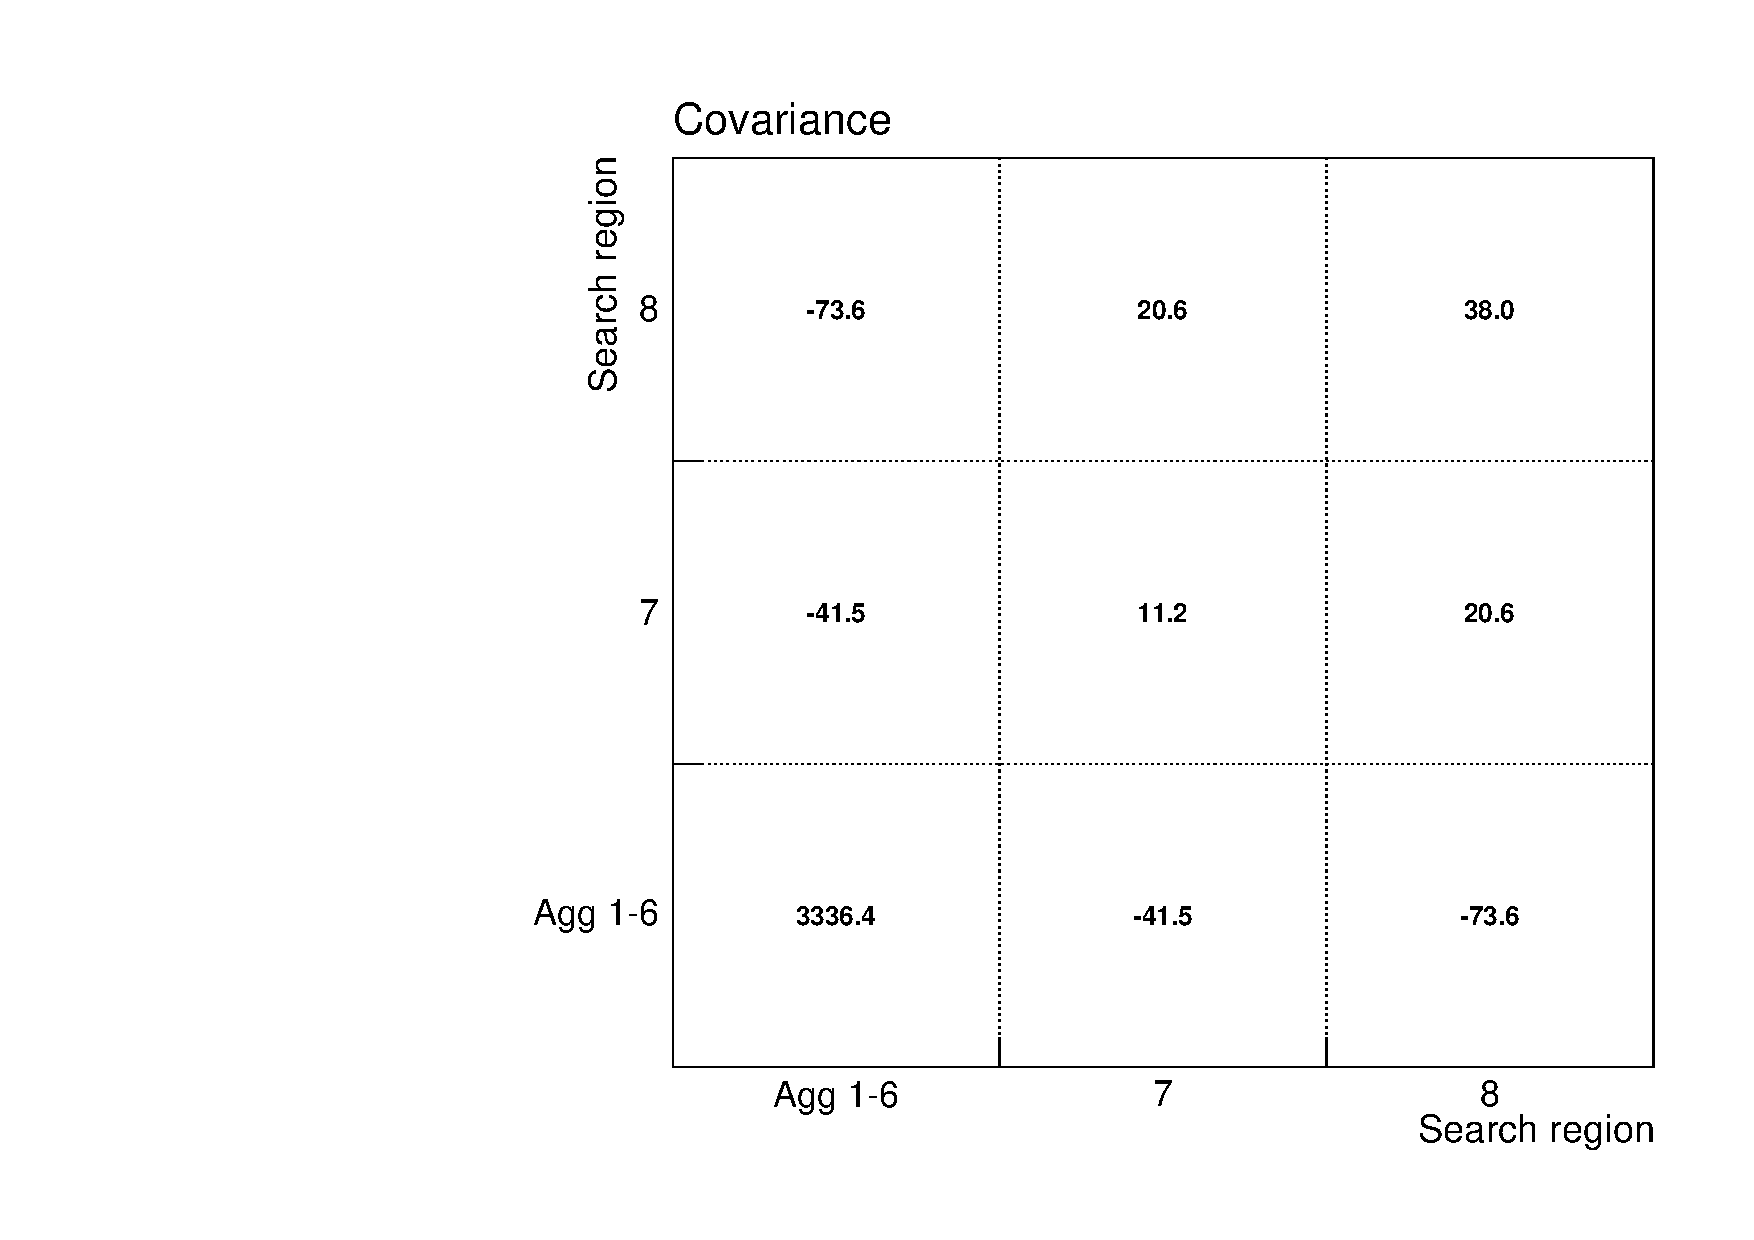
\includegraphics[width=1.5\cmsFigWidth]{figures/agg_htsearch_covariance.pdf}
   \caption{Covariance between the total rate of background contributions expected in each of the aggregated search regions}
   \label{fig:agg-covariance} 
  \end{center}
\end{figure}

Figure~\ref{fig:agg-likelihoodscan} shows the value of $q(\mu)$ as a function of $\mu$. The values when $q(\mu)$ 
is defined using the likelihood of Equation~\ref{eq:full-likelihood} for the nominal signal region, the aggregated signal
regions described above, and considering search regions 7 and 8 only are shown. The aggregated regions show
good agreement compared to the nominal while neglecting the regions 1-6 is shown to introduce a considerable
bias in the estimate of $\hat{\mu}$. In addition, the width of the curve when neglecting these regions is considerably
larger implying a larger uncertainty estimate on $\mu$. This can be expected from the loss of information on
the systematic uncertainties when search regions 1-6 are neglected.

\begin{figure}[hbt]
  \begin{center} 
   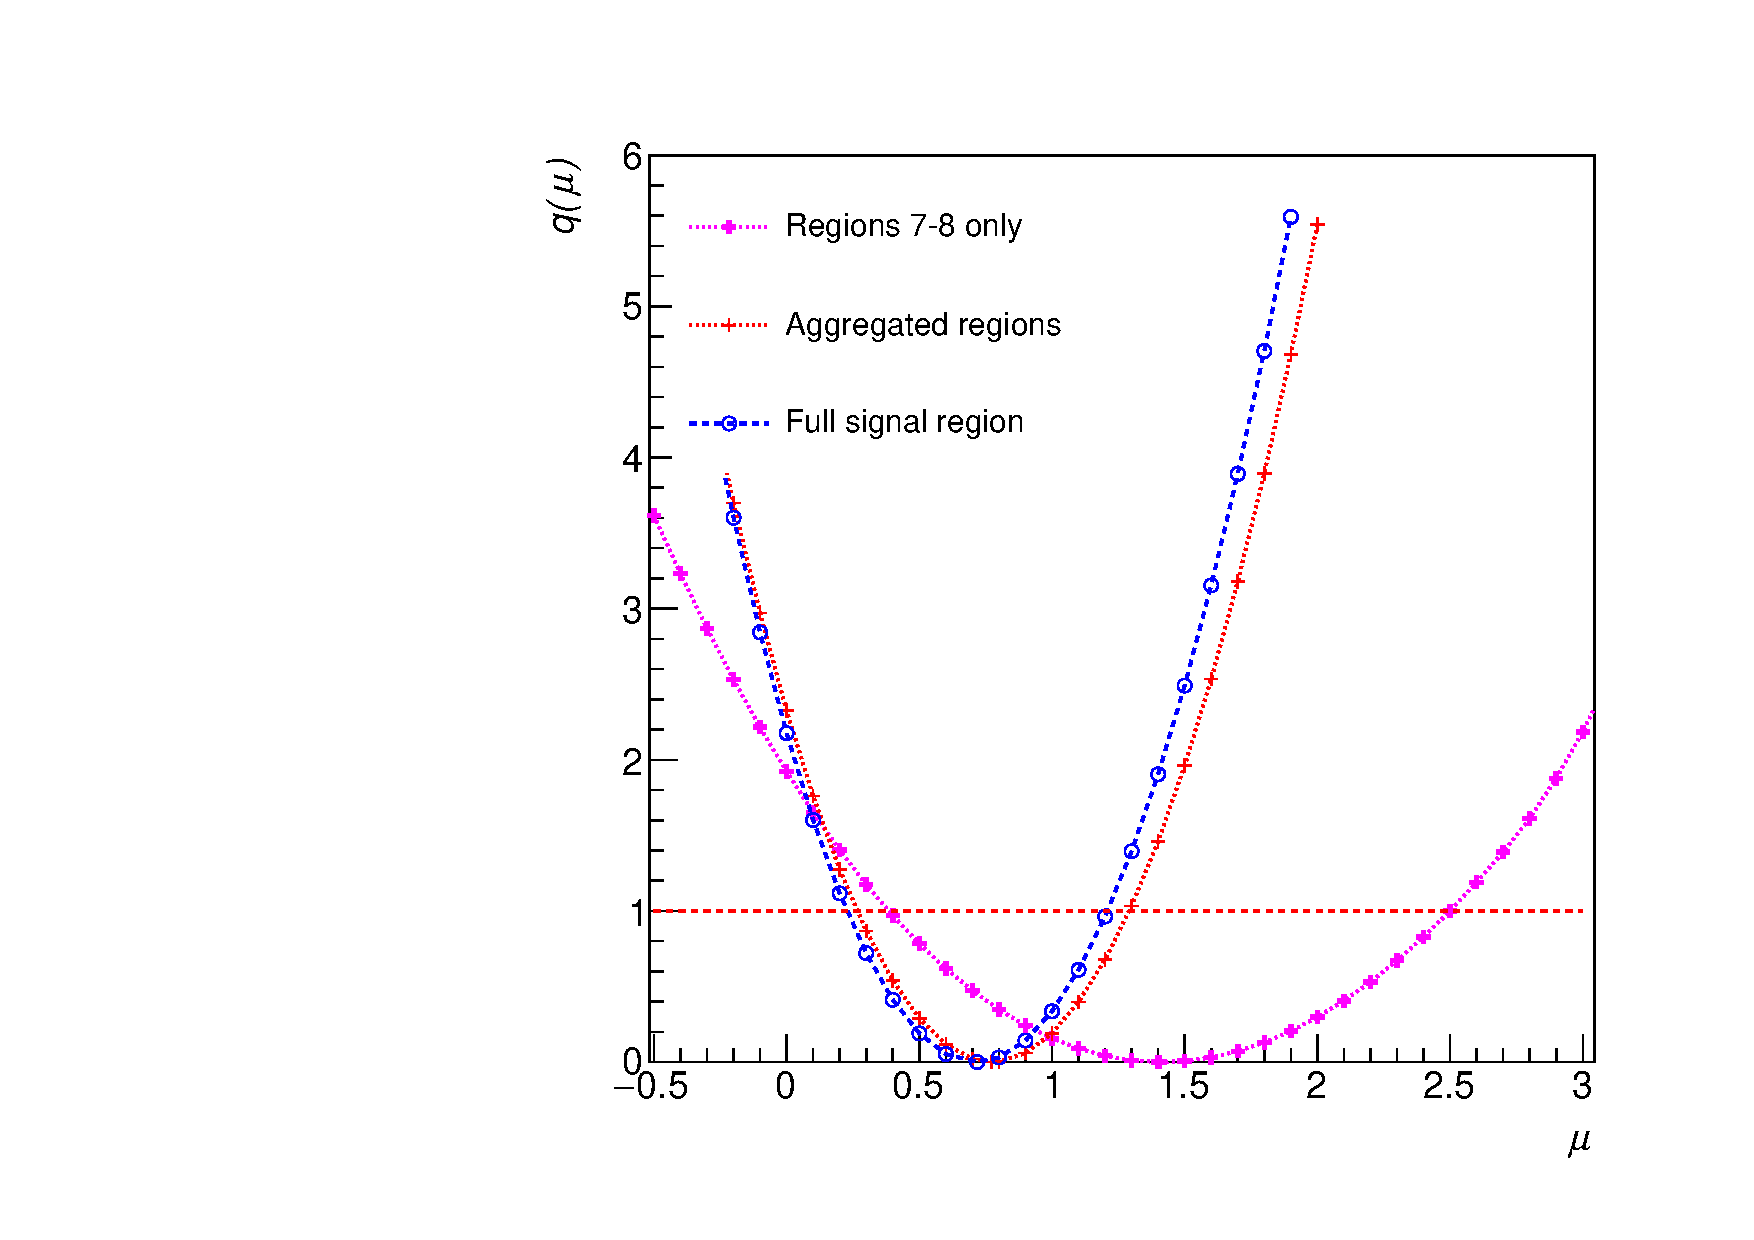
\includegraphics[width=1.5\cmsFigWidth]{figures/r_agg.pdf}
   \caption{The value of $q(\mu)$ defined using the simplified likelihood using the full signal region (), the aggregated signal region (),
   and regions 7-8 only ().}
   \label{fig:agg-likelihoodscan} 
  \end{center}
\end{figure}
